%!TEX root = ../report.tex
\section{Trainingssteuerung}
Trainingssteuerung ist die gewichtete kurz-, mittel- und langfristige Abstimmung und Ausführung aller Planungs-, Trainings-, Kontroll-, Auswertungs- und Lenkungsmaßnahmen eines Trainingsprozesses zur Erreichung der Trainingsziele.
\begin{figure}[H]
  \centering
  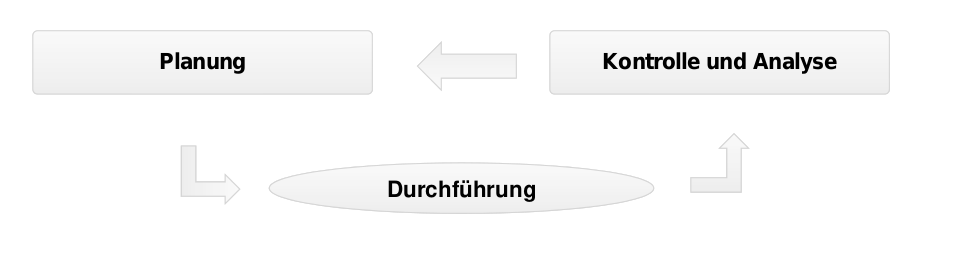
\includegraphics[width=.7\textwidth]{pictures/trainingssteuerung_komponenten.png}
\end{figure}

\subsection{Planung}
\begin{figure}[H]
  \centering
  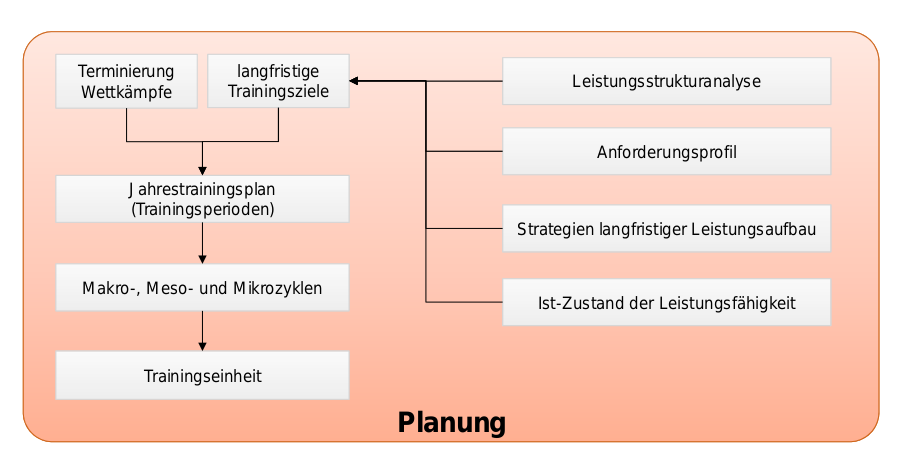
\includegraphics[width=.7\textwidth]{pictures/trainingsplanung_komponenten.png}
\end{figure}
\paragraph{Leistungsstrukturanalyse} Analyse aus welchen Komponenten die Leistung einer Sportart besteht.
Davon werden diejenigen ausgewählt, die besonders entscheidend für den Erfolg sind und werden maximiert.
Die übrigen nur optimiert.\\
\paragraph{Anforderungsprofil} beschreibt wie gut Fähigkeiten auf dem angestrebten Niveau ausgeprägt sein müssen.
Beinhaltet sind:
\begin{itemize}
  \item Leistungsnorm: ist die resultierende Wettkampfleistungen/Teilleistungen
  \item Konditionelle Norm
  \item technisch-taktische Norm
\end{itemize}
\paragraph{Langfristige Traingingsziele} werden mithilfe der Leistungsstrukturanalyse, dem Anforderungsprofil, der Wettkampfanalyse \& der Trainerphilosophie gesetzt.
Folgende fragen sind wichtig:
\begin{itemize}
  \item Ist die Trainierbarkeit gegeben? (Reaktionsschnelligkeit, Kraft)
  \item Lohnt sich das Training? (Abwägung von Niveau, Potential und Zeitbuget)
  \item Ist eine Integration in das Training möglich? (Konkurrenz der verschiedenen Komponenten im Zeitbuget, Wechselwirkungen der Komponenten)
\end{itemize}
\textbf{Planung einer Trainingseinheit}\\
\begin{figure}[H]
  \centering
  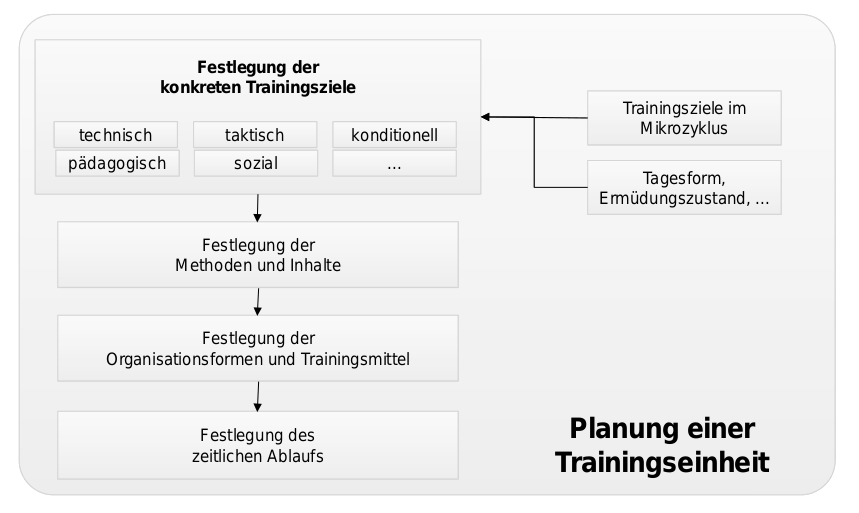
\includegraphics[width=.7\textwidth]{pictures/trainingssteuerung_planung_trainingseinheit.png}
\end{figure}
\begin{figure}[H]
  \centering
  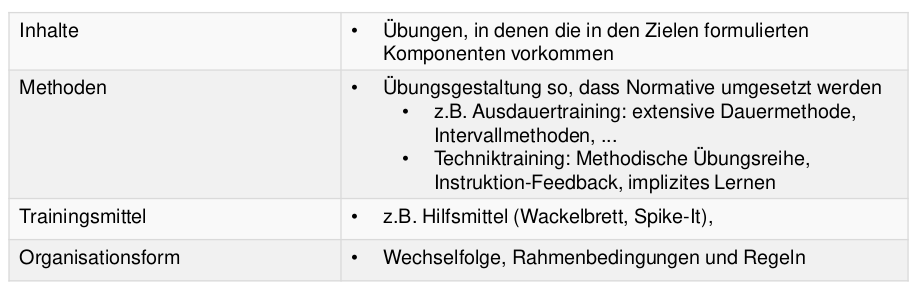
\includegraphics[width=.7\textwidth]{pictures/trainingssteuerung_planung_trainingseinheiten_komponenten.png}
\end{figure}
Zieldefinition:\\
\begin{figure}[H]
  \centering
  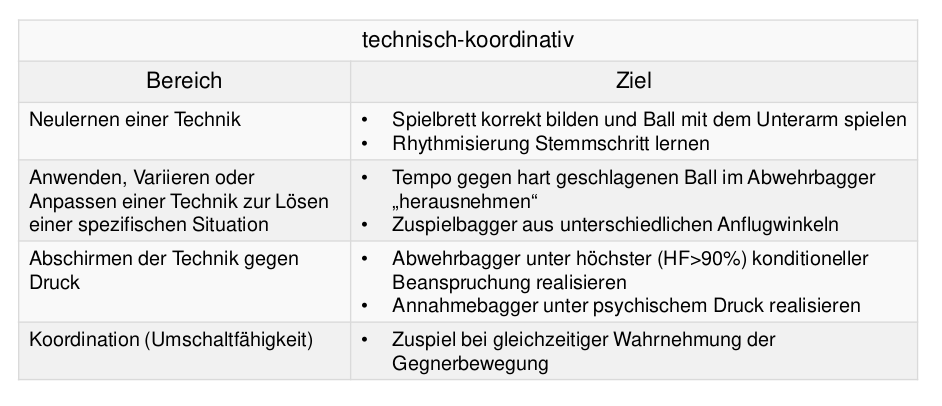
\includegraphics[width=.7\textwidth]{pictures/trainingssteuerung_zieldefinition_koordinativ.png}
\end{figure}
\begin{figure}[H]
  \centering
  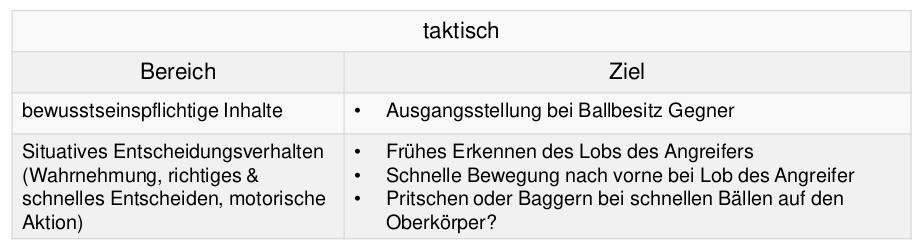
\includegraphics[width=.7\textwidth]{pictures/trainingssteuerung_zieldefinition_taktisch.png}
\end{figure}
\begin{figure}[H]
  \centering
  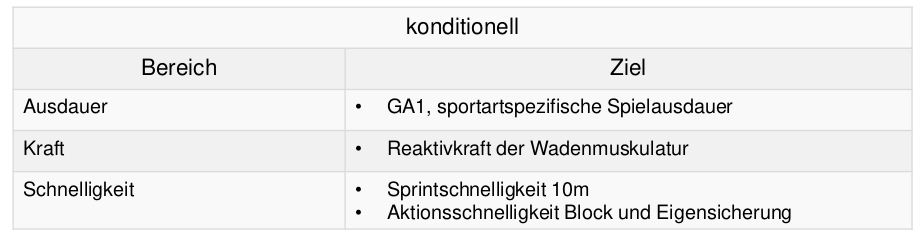
\includegraphics[width=.7\textwidth]{pictures/trainingssteuerung_zieldefinition_konditionell.png}
\end{figure}
Zeitlicher Ablauf einer Trainingseinheit:\\
Der Ablauf ist üblicherweise in drei Teile eingeteilt: Ein einleitender Teil, in dem eine mentale und physische Vorbereitung erfolgt, ein Hauptteil, in dem die Trainingsziele umgesetzt werden sollen und den Ausklang, in dem die Regeneration eingeleitet wird.\\
Im Hauptteil werden zunächst die Trainingsziele umgesetzt, die eher einen erholten Zustand erfordern, wie Schnelligkeit, Koordination oder Reaktion.
Gegen ende des Trainings werden dann vermehrt die anstrengenderen Trainingsziele in betracht gezogen, wie aerobe Ausdauer, Kraftausdauer oder Techniktrainingsabschrimung.

\subsection{Durchführung}
Kritisch überprüfen, ob Training wie geplant abläuft!
\begin{itemize}
  \item Technisch-Taktisch
    \begin{itemize}
      \item Entstehen die benötigten Situationen ausreichend häufig?
      \item Können Techniken in der Situation sinnvoll angewendet werden?
      \item Sind Entscheidungen richtig?
      \item Ist Feedback vorhanden?
    \end{itemize}
  \item Konditionell
    \begin{itemize}
      \item Werden die Normative erreicht (Belastung zu hoch, zu niedrig)? evtl.
      \item Pulskontrolle
      \item Sind Pausen zu lang, zu kurz?
      \item Intensitätssteuerung schwierig -> "mündiger Athlet" (Lenk)
    \end{itemize}
  \item Durchführung ggf.\ verändern (z.B.\ Organisationsform)
\end{itemize}

\subsection{Kontrolle und Analyse}
